\section{The RS03 codec}

\begin{figure}
 \begin{center}
 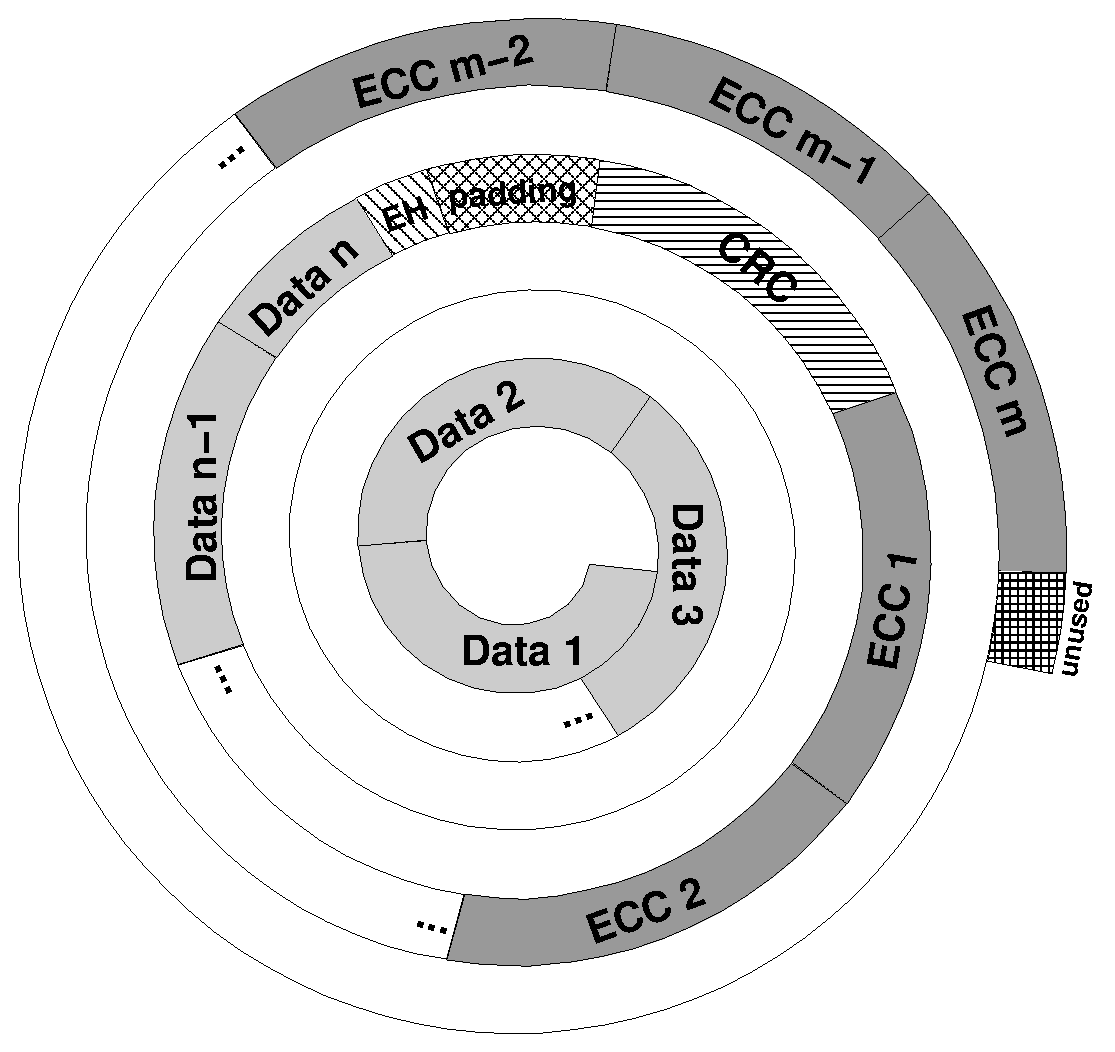
\includegraphics[width=10cm]{spiral-rs03.eps}
 \caption{Physical RS03 layout}
 \label{layout-phy}
 \end{center}
\end{figure}

This section describes the data format of the dvdisaster RS03 Reed-Solomon codec.
RS03 can store parity data either in a separate file or append it to the .iso
image on the same medium. In contrast to its predecessors RS03 is fully multi-threadable.
RS03  is expected to become the default codec soon after its introduction in 
dvdisaster 0.80.

\subsection{Physical layout}

Optical media are recorded as a single long spiral\footnote{Multiple layered
media contain one spiral for each physical layer, but are otherwise conceptually
identical.} of sectors which are indexed beginning with 0. 
The first sector lies at the innermost position of the spiral and 
numbering continues onward to the outside of the spiral.

Reed-Solomon encoding works best when errors are evenly distributed over
all ecc blocks. Therefore we must strive to spread our ecc blocks evenly over
the media surface. To facilitate such distribution, dvdisaster logically
divides the medium into 255 units which are called ``layers'' for historical reasons.
Figure \ref{layout-phy} illustrates how a medium is divided into $n$ data layers,
one CRC layer, and $m$ ecc layers, with $n+m+1 = 255$. Ecc blocks are comprised
by taking one byte from each layer as shown in fig. \ref{layout-logical} on 
the following page.
This distributes the ecc block reasonably good 
over the medium surface.

Layer size is measured in numbers of sectors which are 2048 bytes in size. All
255 layers have the same size. The data layers map exactly 
to the iso image which is to be protected by dvdisaster; 
e.g. the number and sequence of sectors in $Data_1,\ldots,Data_n$
is the same as in the iso image. Two extra sectors are appended to the ISO image
holding the ecc header ``EH''; these are logically treated as a part of the ISO image.
If the ISO image size plus the two EH headers is not an integer multiple
of the layer size, the last (n-th) data layer will be padded accordingly.  

The data layers are followed by a CRC layer. Each CRC layer sector contains a
data structure holding CRC32 checksums for the data sectors plus additional
parameters which were used during the RS03 encoding process.
The data and CRC layers are protected by the
Reed-Solomon parity which is stored in the remaining layers ($ECC_1,\ldots,ECC_m$).
Since the medium capacity is not necessarily an integer multiple of 255, some
unused sectors remain at the end of the medium. These are neither written nor
referenced in any way.

\smallskip

The RS03 data can be stored either directly on the medium or into a separate file.
Figure \ref{layout-phy} shows the first case where ecc data is embedded into the
image; this is also called a ``RS03 augmented ISO image'' in dvdisaster
terminology. 
In the other case a separate error correction file will be created containing
the sectors starting with the EH header. The following discussion is based
on the augmented image case; see section \ref{eccfile} for handling the
file based format.

\subsection{Logical layout}

\begin{figure}
 \begin{center}
 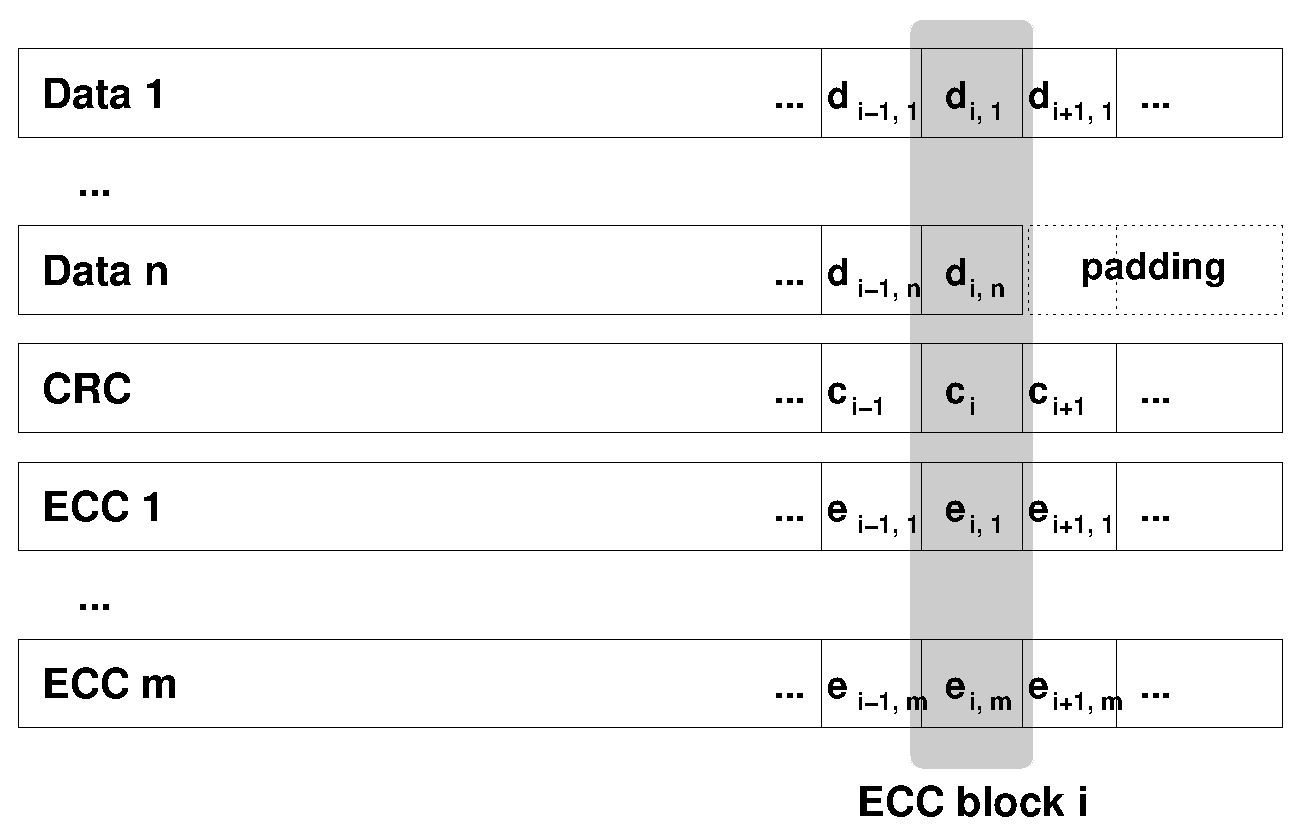
\includegraphics[width=\textwidth]{layer.eps}
 \caption{Logical RS03 layout}
 \label{layout-logical}
 \end{center}
\end{figure}


The relationship between layers and ecc blocks is stated again in the
logical view presented in figure \ref{layout-logical}. Here the 255 layers are
shown in stacked order. From each layer the $i-th$ byte corresponds to the
$i-th$ error correction block. The parity is calculated using $n$ data bytes
$d_{i,1},\ldots,d_{i,n}$ plus the crc byte $c_i$. The resulting $m$ roots of 
the completed Reed-Solomon code are then stored in the 
ecc bytes $e_{i,1},\ldots, e_{i,m}$. 

Since the input iso image plus the two EH sectors is usually not an integer 
multiple of the layer size, the last data layer $data_n$ may contain padding
sectors containing a special signature. The content of the padding sectors
is used in the ecc byte calculation and is written into the augmented image.

\subsection{Calculating the layout for encoding}

\begin{table}
 \begin{center}
 \begin{tabular}{|lrr|}
 \hline
 Medium type &  Maximum size & Layer size \\
 \hline
 CD & 359.424 & 1.409 \\
 DVD 1 layer & 2.295.104 & 9.000 \\
 DVD 2 layers & 4.171.712 & 16.359 \\
 BD 1 layer & 11.826.176 & 46.377 \\
 BD 2 layers & 23.652.352 & 92.754 \\
 \hline
 \end{tabular}
 \caption{Sector size parameters for several media types}
 \label{layout-size-table}
 \end{center}
\end{table}

When encoding with RS03 the layout of the augmented image is fully specified
by two values: the maximum medium size and the iso image size
(from now on, ``size'' always means ``number of 2048K sectors''). \bigskip

Media sizes are hard coded and taken from table \ref{layout-size-table}. Since we need to divide the medium into 255 layers, the layer size
is:
 
\[layer\ size = \left\lfloor\frac{medium\ size}{255}\right\rfloor\]

This allows us to compute the number of data layers needed to cover the iso image plus the ecc header:

\[data\ layers =  \left\lceil\frac{iso\ image\ size + 2}{layer\ size}\right\rceil\]

The number of padding sectors in the last data layer is:

\[padding\ sectors = layer\ size * data\ layers - iso\ image\ size - 2\]

For Reed-Solomon encoding, we will have to encode 

\[n\ data\ bytes = data\ layers + 1\]

and produce the following number of parity bytes:

\[m\ roots = 255 - n\ data\ bytes\]

The RS03 augmented image must fill the medium completely (except for the 
$medium\ size \bmod 255$ sectors  at the end). However for performance
reasons the maximum redundancy is capped to 200\%, or 170 roots. This means
that the ISO image must at least span the first 255-170=85 layers, otherwise
additional padding will be added to fill up the 85 data layers. This situation
is not reflected in the calculations and figure shown above.

\subsection{Re-calculating the layout from defective media}
\label{recover}

In order to recover a defective medium, the values of {\em layer size}
and {\em data layers} need to be determined. The RS03 format allows
for three heuristics with increasing complexity for learning about these
values:

\subsubsection{Using the Ecc Header}

All required information can be obtained from the data structures of the
Ecc Header which is described in appendix \ref{eh}. 
If ecc data is stored in a separate error correction
file, the first 4096 bytes of the ecc file yield the Ecc Header.
Otherwise, let $n$ be the size of the ISO file system which
can be obtained from the ISO file system master block. Then the 
Ecc Header is typically found in the RS03-augmented image at sectors $n,n+1$ 
or at $n+150,n+151$ (due to padding inserted by some popular CD-R  mastering
software). \smallskip

If the ISO file system master block is unreadable, the Ecc Header
can be identified by its characteristic signature and checksum. 
If the Ecc Header is encountered during reading of the defective medium 
it might be worthwhile to generate a tentative ISO master block in the image
file. This would speed up future processing of the image; however current
implementations of dvdisaster do not yet implement this feature.

\subsubsection{Using the CRC layer}

Each CRC layer sector contains a data structure which not only holds the
CRC32 checksums but also a copy of important parameters from the Ecc header
(see section \ref{crc} for details). CRC sectors can be easily recognized
by looking for their signature and checksum while scanning the medium image.
If dvdisaster finds a valid CRC sector and the Ecc header is defective,
a tentative Ecc header is written to the image to speed up further
operations on the image file.

However it should be noted that since all CRC sectors are stored 
consecutively on the medium, they can easily be wiped out by a large
defective region on the medium. Therefore, another heuristic exists
for learning about the RS03 layout.

\subsubsection{Evaluating the Reed-Solomon code}
\label{recover-rs}

If neither the Ecc Header nor any CRC sectors are readable
the RS03 layout can be determined by the following heuristic.

First, the medium size is determined from table \ref{layout-size-table}.
This is always possible as long as the drive will recognize the medium at all.
Since the layer size is $\left\lfloor\frac{medium\ size}{255}\right\rfloor$,
the location of the 255 layers on the medium is now known. The remaining task is to find
out the redundancy of the Reed-Solomon code, e.g. how many layers contain
roots for the RS code.

\bigskip

Taking the {\em i-th} sector from each layer will produce a valid error 
correction block, but with unknown redundancy. As RS03 will create redundancies 
using 8 to 170 roots, we employ a brute-force approach by evaluating
the Reed-Solomon code for $8..170$ roots. If the error correction
is successful for $n$ roots and the sector from layer {\em 255-1-n} yields
the CRC data structure, the correct number of roots has been found.

\medskip

In reality, not all 162 combinations of roots need to tested since additional
information can be exploited:

\begin{enumerate}
\item If the sector from layer {\em 255-1-n} is present/readable,
we do not need to test for $n$ roots any further: Encoding with $n$ roots would
have produced a CRC sector in this place.
\item If the number of erasures (as indicated by unreadable sectors) is higher
than $n$, we can trivially skip the RS decoding. We might have to test another
set of 255 sectors though if testing for all other numbers of roots fails as well.
\end{enumerate}

Criterion 1) should quickly narrow down the possible numbers of roots
in the average case, e.g. when enough redundancy is available for recovering the medium.
Worst case behaviour of trying each ecc block for 8..170 roots is likely to appear only
when the medium is unrecoverable, e.g. when more sectors are damaged than the 
Reed-Solomon code can correct.

\subsection{Contents of the CRC layer}
\label{crc}

Each sector of the CRC layer contains the data structure shown in
appendix \ref{crc-block}. Following the numbering from figure \ref{layout-logical},
CRC sector $c_i$ contains the CRC32 checksums for data sectors $d_{j,1},\ldots,d_{j,n}$
with $j = (i+1)\bmod\ layer\ size$. The purpose of this offset is to have
the error correction of ECC block $i$ recover the CRC checksum for the next 
ECC block $i+1$. In case of readable but corrupted sectors this will keep the
error correction in erasure mode and therefore save precious redundancy (the
RS code can recover twice as much errors when the location of defective data
is known). \medskip

Checksums for data sector $d_{j,k}$ are stored in array element
CrcBlock-$>$crc[k]. Unused array elements are set to zero.
The remaining contents of the CRC sector structure provide 
configuration and layout information; see appendix \ref{crc-block} for details.

\subsection{Encoding the ecc layers}

Encoding the error correction information
 requires reading and buffering of at least
255 sectors comprising the ecc block
(see fig. \ref{layout-logical} for a definition of the ecc block).
A possible encoding algorithm
might process each ecc block at a time. For each ecc block $i$
it would do the following: \smallskip

First, the $n$ data sectors $d_{i,1},\ldots,d_{i,n}$ of the ecc block
are read in. The CRC layer 
sector $c_i$ is initialized, filled in with checksums 
generated by processing the previous ecc block, and completed
by calculating its own checksum {\em selfCRC}. Unused portions of $c_i$
remain zero. Afterwards the
CRC32 checksums of $d_{i,1},\ldots,d_{i,n}$ are calculated
and stored away using the same buffering mechanism. Since the hand-over of
CRC checksums between ecc blocks is the only place where RS03 does 
not fully parallelize, data sector I/O and CRC32 caching needs to be 
carefully thought out in multithreaded implementations. \medskip


Once $d_{i,1},\ldots,d_{i,n}$ and $c_i$ have been prepared, 
2048 sets of a  RS(255,k) code (with $k=255-n-1$) are calculated by 
looping over the 2048 bytes of the ecc sectors. If $l$ denotes
a certain byte position between $0,\ldots,2047$ in the ecc block
sectors, then the {\em l-th} byte from $d_{i,1},\ldots,d_{i,n},c_i$
is retrieved and fed into the RS(255,k) encoder. The resulting
parity bytes $p_1,\ldots,p_m$ are stored in byte position $l$ of the
ecc layer sectors $e_{i,1},\ldots,e_{i,m}$. When all 2048 bytes
of the ecc block sectors have been processed the ecc layer sectors
can be written out; either into the error correction file or into
the RS03 augmented image. \medskip

The RS(255,k) encoder is the same for RS01, RS02 and RS03. See
appendix \ref{rs} for the parameters used in the encoder.

\subsection{Encoding as a separate error correction file}
\label{eccfile}

If the image size is too close to the medium capacity, not enough
space is left for augmenting the image with redundancy. dvdisaster
will refuse to augment images when there is insufficient space
for at least 8 roots. Creating images with less than 43 roots
(20\% of redundancy) will trigger a warning that the error correction
capacity may be too low. In those cases, storing the error correction
information in a separate file comes as an alternative.

\medskip

RS03 error correction files (``ecc files'')
contain the same error correction information
and layout as in the augmented image case, with the following differences:

\paragraph{Omittance of data padding sectors.} While the image format
shown in figures \ref{layout-phy} and \ref{layout-logical}
 may contain padding sectors between the ecc header and the CRC layer,
those sectors are not written into the ecc file.
The padding sectors are however required during encoding and
decoding, e.g. they need to be virtually created in memory 
when processing the respective ecc blocks. 
Therefore an ecc file providing {\em nroots} of redundancy
will contain {\em 2 + (nroots+1) * layer size} sectors.
Physically it will contain the ecc header, then the CRC layer 
and finally the {\em nroots} ecc layers. In contrast to the
augmented image case, the ecc header {\em is not part of an ecc
  block} and can therefore not be recovered
by the error correction. If the ecc header is lost in an ecc file,
its contents can be reconstructed from a still existing block
in the CRC layer and then be rewritten accordingly.

\paragraph{Freely chooseable redundancy.} In the augmented image case
the redundancy is always chosen to fill up the medium completely.
For ecc files the redundancy can be freely chosen by the user between
 8 roots (3.2\%) and 170 roots (200\%). Encoding with more than 170 roots
is technically possible, but run-time requirements get out of proportion;
hence the selectable redundancy is capped at 200\%.

\medskip

As a consequence of the variable redundancy the ecc file layout can only
be determined by looking at the ecc header or CRC sectors. The strategy
of experimentally evaluating the Reed-Solomon code (see sub 
section \ref{recover-rs}) however can not be applied to ecc files since
neither the size of the padding area nor the original size of the 
possibly truncated image and ecc files can be determined. \medskip

To see whether this is really a limiting factor we look
at the typical outcome of recovering a single file from a defective
medium:

\begin{itemize}
\item The ecc file is fully read, but random sectors are damaged.
\item The ecc file is truncated to the position of the first read error.
\end{itemize}

In both scenarios it is highly likely that at least one CRC sector survives
at the beginning of the file; in that case the error correction will not
only recover the image but also repair the ecc file into its original state.

\bigskip

Although this gives RS03 ecc files good chances to remain functional even
when being partly damaged, it is highly recommended to store ecc files 
only on media which are themself being protected by dvdisaster. 
ISO and UDF file systems
do not have sufficient redundancy for their meta data (e.g. directory
structures). If such meta data becomes unreadable a significant
number of files may become completely inaccessible. 
Please note that this is a
general weakness of file-based data protection and recovery: The
meta data is not part of any file and can therefore not be protected by
any error correction data put inside the file(s). 
\smallskip
This is the also the simple reason why we did not use tools like PAR2 
and developed dvdisaster instead; 
the image-based approach of dvdisaster protects
both files and meta data.
